


\chapter{Seam carving algorithm.}

\section{Presentation of the algorithm.}


At the beginning, the seam carving algorithm is used in order to reduce the size of an image and keep some proportion of the image. The main idea of this algorithm is to find the path in an image which have the least importance and automatically remove them in order to resize the image \cite{avidan2007seam}.

The following figure show what kind of result can be expected and the different step of the algorithm:

\begin{figure}[H]
\centering
    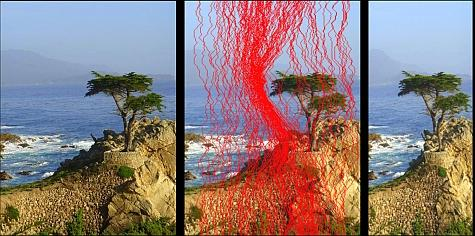
\includegraphics[scale=1,angle=0]{Images/ankit-rahul.jpg}
    \caption{Example of the seam carving algorithm, coming from the website \textit{http://courses.cs.washington.edu/courses/cse557/08wi/projects/final/artifacts.html}.}
    \label{fig:ankit-rahul}
\end{figure}


Nevertheless, it can be used in this project in order to find a approximation of the frequency law which compose a signal. In the time frequency representation, the different laws which compose the signal represent a path in the image and we can use this algorithm in order to find an empiric expression $f(t)$.
The main purpose of those articles \cite{barnwal2013doppler} \cite{couvreur1997doppler} \cite{cevher2009vehicle} is to present how this algorithm can be implement in order to find the speed of an object thanks to the Doppler effect but it can be use here in order to find the frequency laws which compose the signal. 

The seam carving algorithm can be express by the following line:

\begin{algorithm}[H]
  \caption{SEAM CARVING algorithm }
  
  \textbf{Inputs}% Inputs section
  \begin{algorithmic}[1]
    \STATE Matrix TFR
    \STATE Vector $T$ time
    \STATE Vector $F$ frequency
  \end{algorithmic}
  \bigskip

  \textbf{Output}% Output section
  \begin{algorithmic}[1]
    \STATE Vector Value $f(t)$ of the first frequency law found
  \end{algorithmic}
  \bigskip
  
  \textbf{Initialization}% Initialization section
  \begin{algorithmic}[1]
   	\STATE $init\gets 0$
   	\STATE $i\gets 0$
	\STATE $k\gets zeros(len(t),1)$
  \end{algorithmic}
  
  
  \textbf{Algorithm}% Inputs section
  \begin{algorithmic}[1]
  %\textit{Construction of the path}%
	\WHILE{i<len of T}

	 	%\textit{Initialization, either at the beginning or if no law has been found yet.}%
	 	\IF{i==0 or init == 0}
     	  	\STATE $peakind\gets$ peak of the vector TFR$[:,i]$
     	
	 	
	 	%\textit{if at least one peak has been found}%
  	 		\IF{$len(peakind)!=0$}
				\STATE $k[i]\gets peakind[0]$
				\STATE $init\gets 1$
				
	 	
			\ELSE{}
				%\textit{else if a maximum has been found}%
				\IF{max(TFR[:,i])!=0)}
					\STATE $k[i]\gets$ indice of the maximum of the vector $TFR$[:,i]
					\STATE $init\gets 1$
				\ENDIF
			\ENDIF
				
		%\textit{A law has been found and we build the path step by step according to the neighbourhood of the current point.}%
		\ELSE
			\STATE $Indice\gets$ the value of j, when the values $TFR$[k[i-1]+j,i] is maximize, for j in $[-1,0,1]$
			\STATE $k[i] = k[i-1] + Indice$
	 	\ENDIF
	 	\STATE $i++$
	\ENDWHILE 
	
	
  return $k$


  \end{algorithmic}
\end{algorithm}

\section{Application on a Doppler signal.}

We can apply easily this algorithm on a Doppler signal. Let suppose that an object is moving toward an observer and it is sending a wave (sound for example). The frequency of the signal is changed because of the movement of this object. The following figure shows how the signal is affected by the movement:

\begin{figure}[H]
\centering
    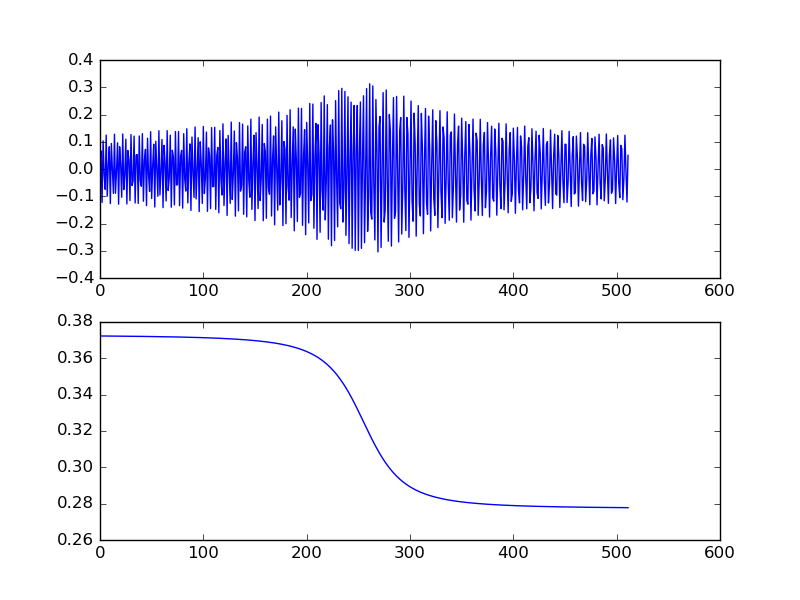
\includegraphics[scale=0.6,angle=0]{Images/doopler_signal.png}
    \caption{Time representation and instantaneous frequency of the signal send.}
    \label{fig:doopler_signal}
\end{figure}

The next figure show the time-frequency representation of the signal:

\begin{figure}[H]
\centering
    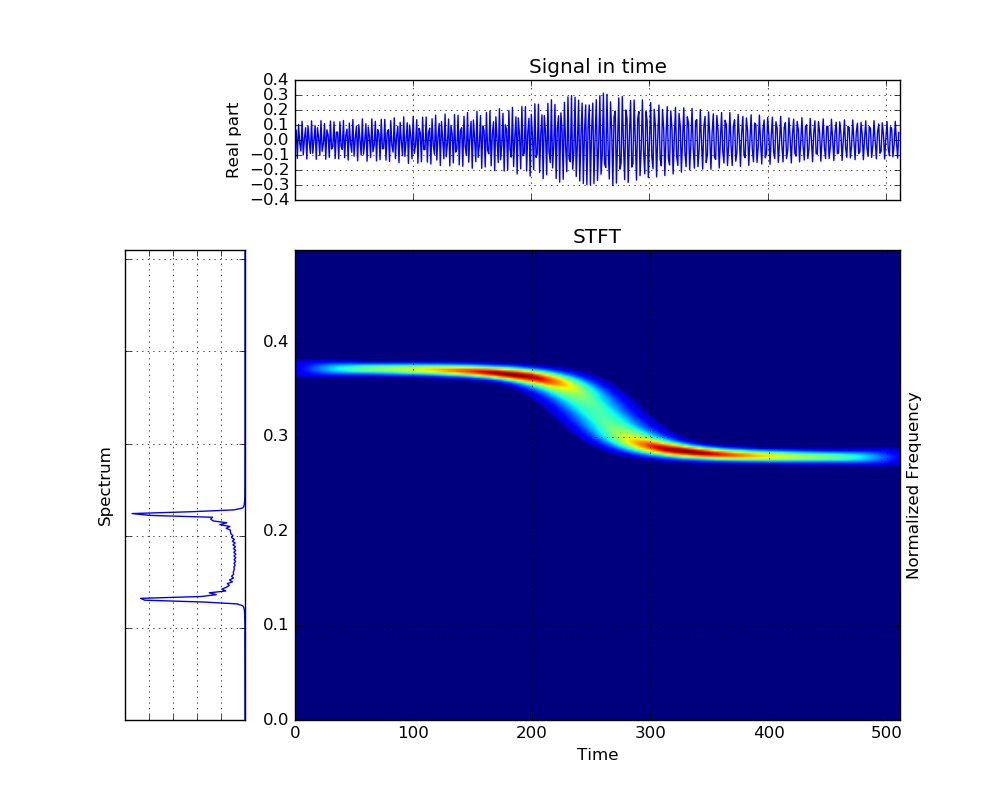
\includegraphics[scale=0.6,angle=0]{Images/doopler_signal_spec.png}
    \caption{Time/Frequency representation of the signal send.}
    \label{fig:doopler_signal_spec}
\end{figure}

Thanks to some tools coming from the image processing, we can improve this result in order to keep only the relevant points which contain information:

\begin{figure}[H]
\centering
    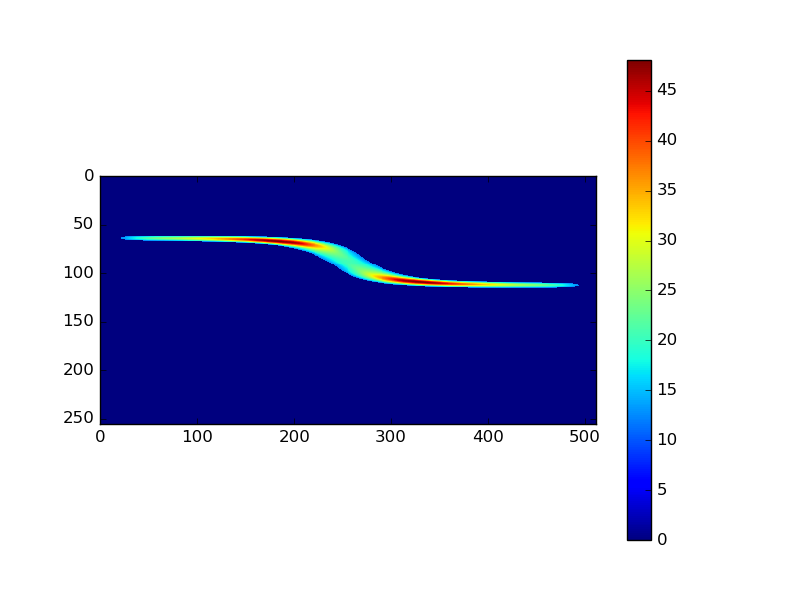
\includegraphics[scale=0.6,angle=0]{Images/varseuil_signal.png}
    \caption{Time/Frequency representation of the signal send after treatment.}
    \label{fig:varseuil_signal}
\end{figure}

Finally, when we use the seam carving algorithm, we achieve to get this result:

\begin{figure}[H]
\centering
    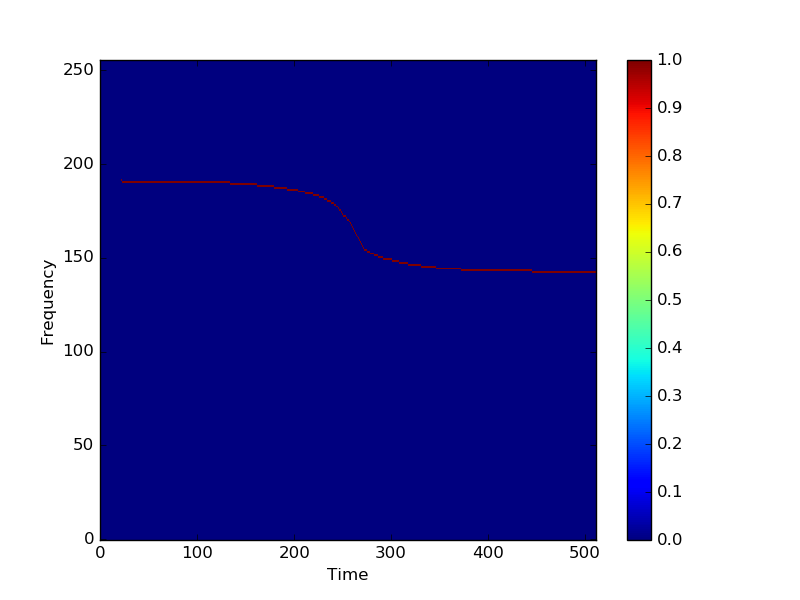
\includegraphics[scale=0.6,angle=0]{Images/doopler_signal_esti.png}
    \caption{Time/Frequency representation of the signal send after treatment.}
    \label{fig:doopler_signal_spec}
\end{figure}

The last part is to use interpolation algorithm such as fit spline interpolation in order to find an approximation of the law found. The following figure shows how the fit spline interpolation can provide some results:

\begin{figure}[H]
\centering
    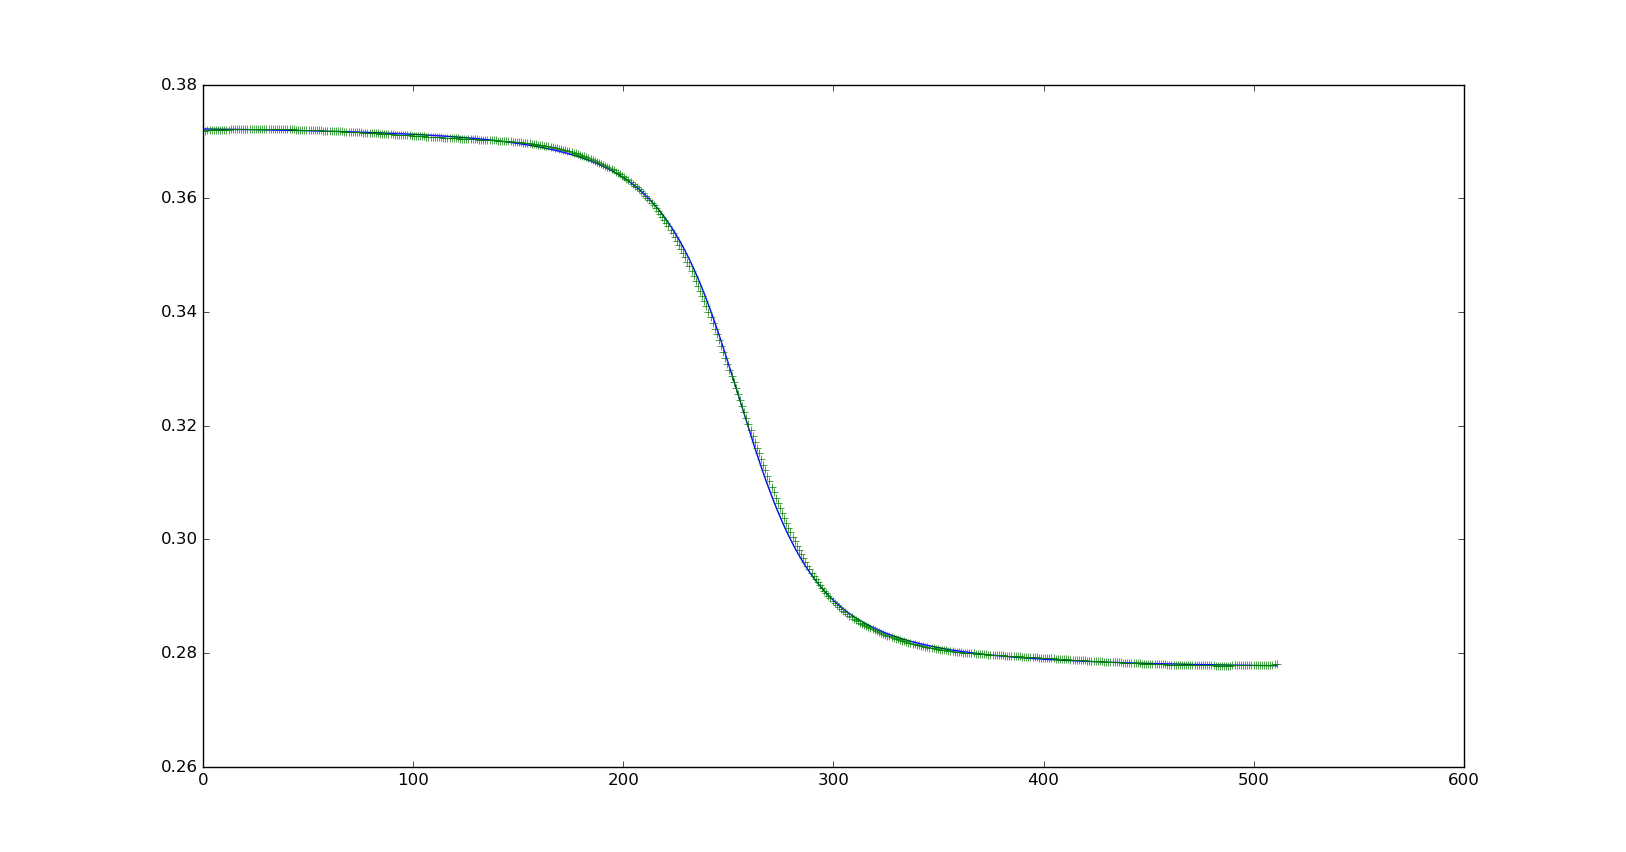
\includegraphics[scale=0.35,angle=0]{Images/spline_pour_la_loi_de_frequence_trouvee.png}
    \caption{Spline interpolation result. In green the value of the interpolation and in blue the value of the law found}
    \label{fig:spline_pour_la_loi_de_frequence_trouvee}
\end{figure}

Nevertheless, the result given by this method can be disturbed by the beginning of the signal. For example, the following figure shows how the first values of the law found can impact the interpolation.

\begin{figure}[H]
\centering
    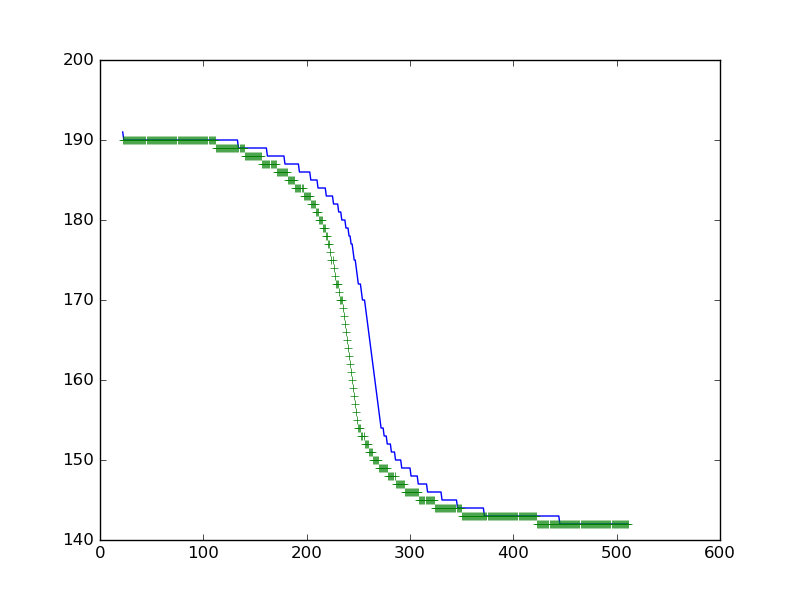
\includegraphics[scale=0.6,angle=0]{Images/spline_pour_la_loi_de_frequence_trouvee2.png}
    \caption{Spline interpolation with bad result. In green the value of the interpolation and in blue the value of the law found}
    \label{fig:spline_pour_la_loi_de_frequence_trouvee2}
\end{figure}

As the different part have shown, we have now all the tools needed in order to create and then analyse any kind of signal, including the signal details in the introduction.

\chapter{Application to our project.}

In this part, we will apply all the result of the previous part in order to analyse understand the signal generate by the cylinder as it was explain in the introduction.

\section{A first application.}

Let consider a cylinder which \textbf{radius don't change through time} but it's moving according to the following figure.

\begin{figure}[H]
\centering
    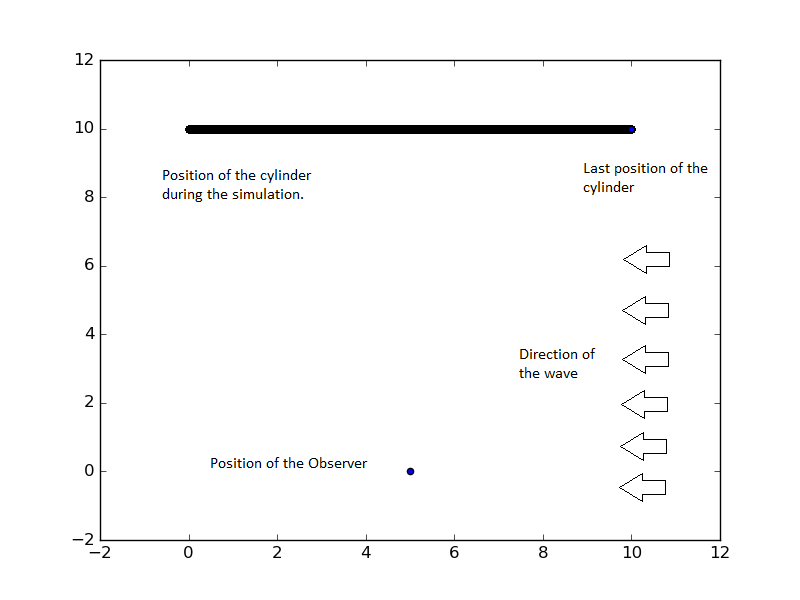
\includegraphics[scale=0.6,angle=0]{Images/Position.png}
    \caption{First situation studied. The object is moving linearly.}
    \label{fig:moving linearly}
\end{figure}

The following figure shows the spectrogram obtain after we analyse the signal without its means.

\begin{figure}[H]
\centering
    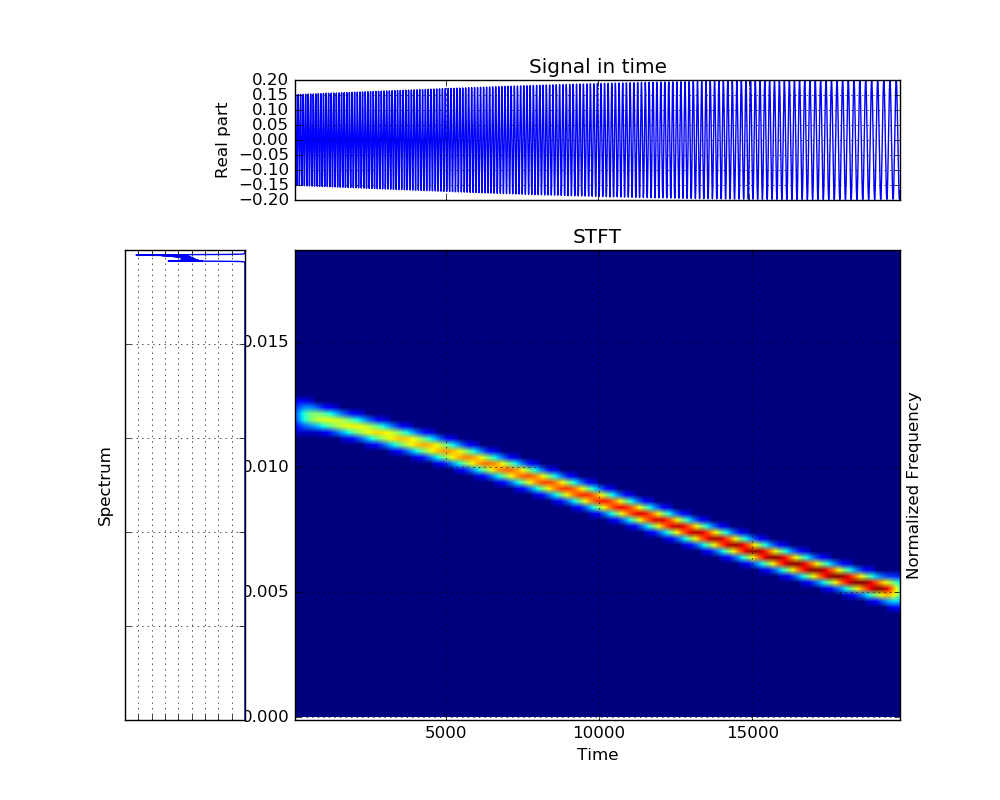
\includegraphics[scale=0.6,angle=0]{Images/SpectrogramObjMov.png}
    \caption{Spectrogram of an object moving linearly.}
    \label{fig:SpectrogramObjMov}
\end{figure}

And this figure show the result of the seam carving algorithm:

\begin{figure}[H]
\centering
    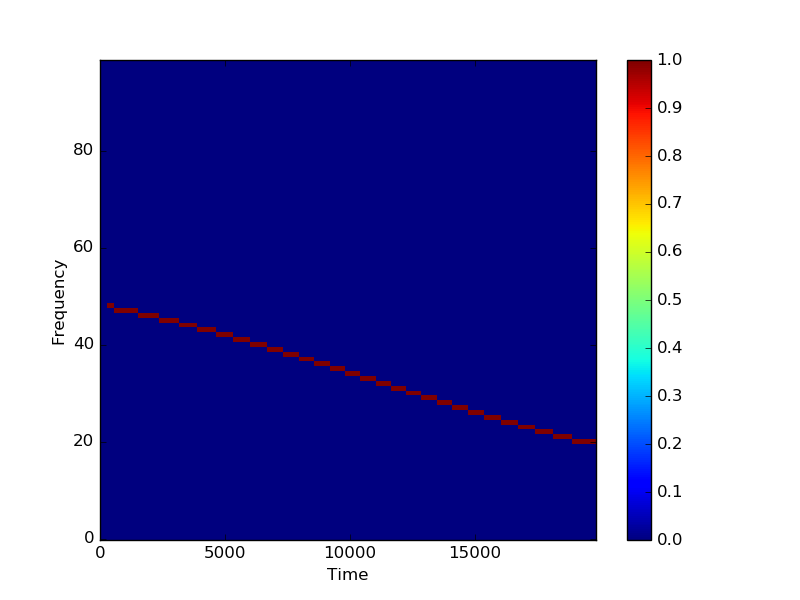
\includegraphics[scale=0.6,angle=0]{Images/SpectrogramObjMov_LawFound.png}
    \caption{Seam carving application.}
    \label{fig:SpectrogramObjMov_LawFound}
\end{figure}

As you can see, we are in the same configuration as the Doppler signal we have studied in the previous part. There is a frequency which value received by the observer is disturbed by the movement. Futhermore, the seam carving apply perfectly to this kind of figure as the figure \label{SpectrogramObjMov_LawFound} shows it.

\section{Application in view to a verification in the anechoic chamber.}

The school ENSTA Bretagne has a anechoic chamber in which we can simulate the field generate and scatter by object but we can only give a circular movement to those object. Thanks to the code we have created, we know that the wave scatter and it's time frequency representation will be:

\begin{figure}[H]
\centering
    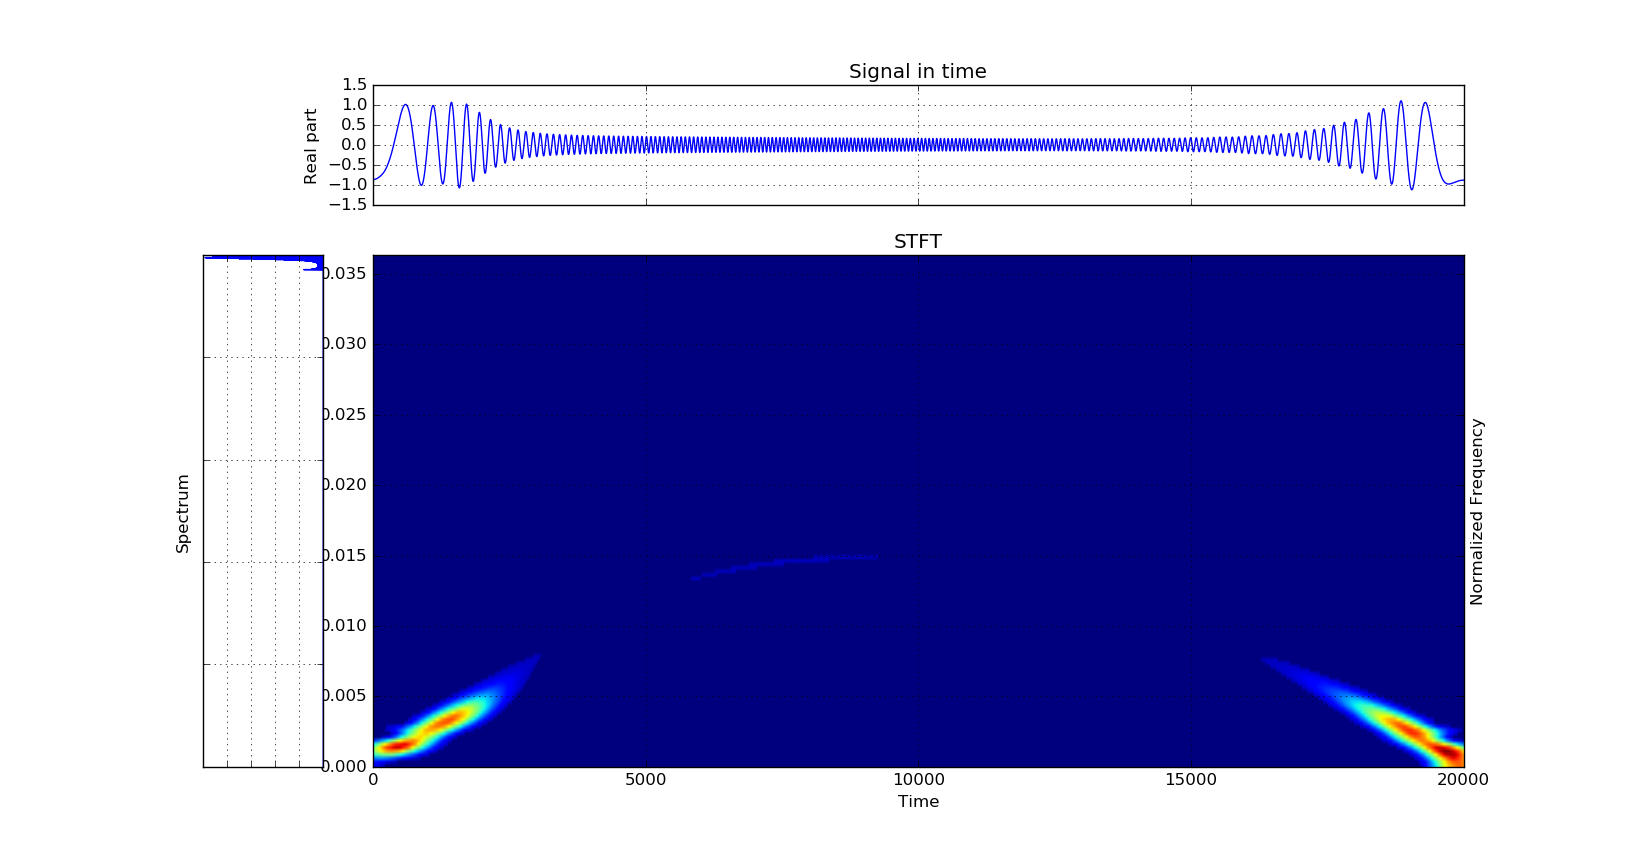
\includegraphics[scale=0.35,angle=0]{Images/TFR3.png}
    \caption{Time frequency representation of a cylinder with a circular movement.}
    \label{fig:TFR3}
\end{figure}

The partial sinusoid we can see in this time frequency representation is conformed to the theory but the signal contains too much energy when it's close to the observer which explains why we don't see all the curve.

Thanks to this code, we can generate easily any signal for any object and we can check if the theoretical results are corroborated by the experimental results.

\section{Application to object which form change through time.}

According to the document coming from the supervisors, if we consider a single cylinder which form change through time, we should get time-frequency representation like this one:

\begin{figure}[H]
\centering
    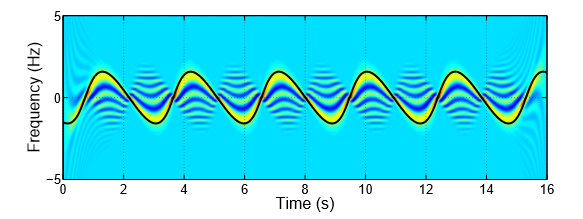
\includegraphics[scale=0.6,angle=0]{Images/TFRExpected.png}
    \caption{Time frequency representation expect. The frequency received have a periodic behaviour.}
    \label{fig:TFRExpected}
\end{figure}

Nevertheless, even with a lot of test, we only get result like this one:

\begin{figure}[H]
\centering
    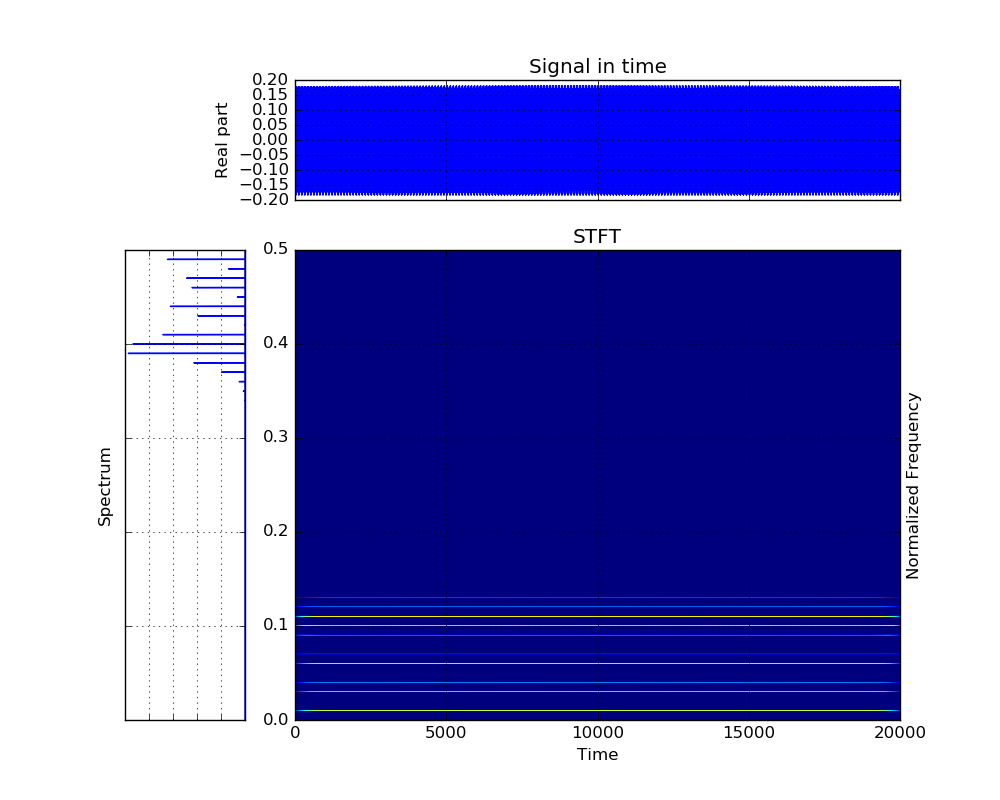
\includegraphics[scale=0.6,angle=0]{Images/Objx3y10.png}
    \caption{Time frequency representation of a cylinder with a sinusoidal variation of its radius.}
    \label{fig:Objx3y10}
\end{figure}

As you can see, we have the fundamental and the harmonic of the original signal which are present in this time frequency representation. But the form changing seems to don't have impact on those law frequency during time.

\chapter*{Conclusion}
\bigskip

All the different part which have been realized during this project very good result and can be easily reused by anybody.
Most of them can be easily use for the signal we wanted to analyse. Nevertheless, the fact that the impact of the variation of the radius of the cylinder have not been seen is regretful.